%%%%%%%%%%%%%%%%%%%%%%%%%%%%%%%%%%%%%%%%%
% a0poster Landscape Poster
% LaTeX Template
% Version 1.0 (22/06/13)
%
% The a0poster class was created by:
% Gerlinde Kettl and Matthias Weiser (tex@kettl.de)
% 
% This template has been downloaded from:
% http://www.LaTeXTemplates.com
%
% License:
% CC BY-NC-SA 3.0 (http://creativecommons.org/licenses/by-nc-sa/3.0/)
%
%%%%%%%%%%%%%%%%%%%%%%%%%%%%%%%%%%%%%%%%%

%----------------------------------------------------------------------------------------
%	PACKAGES AND OTHER DOCUMENT CONFIGURATIONS
%----------------------------------------------------------------------------------------

\documentclass[a0,landscape]{a0poster}

\usepackage{multicol} % This is so we can have multiple columns of text side-by-side
\columnsep=100pt % This is the amount of white space between the columns in the poster
\columnseprule=3pt % This is the thickness of the black line between the columns in the poster

\usepackage[svgnames]{xcolor} % Specify colors by their 'svgnames', for a full list of all colors available see here: http://www.latextemplates.com/svgnames-colors

\usepackage{times} % Use the times font
%\usepackage{palatino} % Uncomment to use the Palatino font

\usepackage{graphicx} % Required for including images
\graphicspath{{figures/}} % Location of the graphics files
\usepackage{booktabs} % Top and bottom rules for table
\usepackage[font=small,labelfont=bf]{caption} % Required for specifying captions to tables and figures
\usepackage{amsfonts, amsmath, amsthm, amssymb} % For math fonts, symbols and environments
\usepackage{wrapfig} % Allows wrapping text around tables and figures
\usepackage[T1]{fontenc}
\usepackage[utf8]{inputenc}
\usepackage{authblk}
\usepackage{color, amssymb, epsfig, graphicx, bm, amsmath, caption, subcaption, enumerate, graphicx,, setspace,listings}
\usepackage{titlesec}


\definecolor{uwred}{RGB}{197, 5, 12}
\definecolor{jhblue}{RGB}{0,38,73}

\titlespacing{\section}{5pt}{2pt}{8pt}
\titlespacing{\subsection}{5pt}{2pt}{8pt}
\begin{document}

%----------------------------------------------------------------------------------------
%	POSTER HEADER 
%----------------------------------------------------------------------------------------

% The header is divided into three boxes:
% The first is 55% wide and houses the title, subtitle, names and university/organization
% The second is 25% wide and houses contact information
% The third is 19% wide and houses a logo for your university/organization or a photo of you
% The widths of these boxes can be easily edited to accommodate your content as you see fit

\begin{minipage}[b]{0.55\linewidth}
\veryHuge \color{uwred} \textbf{Global PCA of Local Moments} \color{jhblue}\\ % Title
\Huge\textit{With Applications to MRI Segmentation}\\[1cm] % Subtitle
\huge \textbf{Jacob M. $\text{Maronge}^{\text{\large1, 2}}$, John $\text{Muschelli}^{\text{\large3}}$, Ciprian M. $\text{Crainiceanu}^{\text{\large3}}$}\\ % Author(s)
\LARGE $^{\text{\large1}}$University of Wisconsin - Madison, Department of Statistics\\
\LARGE $^{\text{\large2}}$University of Wisconsin - Madison, Department of Biostatistics and Medical Informatics\\  % University/organization
\LARGE $^{\text{\large3}}$Johns Hopkins Bloomberg School of Public Health, Department of Biostatistics
\end{minipage}
%
\begin{minipage}[b]{0.25\linewidth}
\color{DarkSlateGray}\Large \textbf{Contact Information:}\\
Jacob M. Maronge\\
Department of Statistics\\ % Address
University of Wisconsin - Madison\\
1300 University Ave, Madison, WI, 53706\\\\
Email: \texttt{jmmaronge@gmail.com}\\ % Email address
Website: \texttt{https://jmmaronge.github.io}
\end{minipage}
%
\begin{minipage}[b]{0.19\linewidth}

\includegraphics[width=23cm]{logo.png} % Logo or a photo of you, adjust its dimensions here
\end{minipage}

\vspace{1cm} % A bit of extra whitespace between the header and poster content

%----------------------------------------------------------------------------------------

\begin{multicols}{3} % This is how many columns your poster will be broken into, a poster with many figures may benefit from less columns whereas a text-heavy poster benefits from more

%----------------------------------------------------------------------------------------
%	ABSTRACT
%----------------------------------------------------------------------------------------

\color{black} % Navy color for the abstract

\normalsize{\section*{\center{\color{uwred}Abstract}}}
\noindent We are interested in describing the information contained in local neighborhoods, and higher moments of local neighborhoods, of complex multimodal imaging techniques at the population level. This is problematic because of the size of medical imaging data. We propose a simple, computationally-efficient approach for representing the variation in multimodal images using the spatial information contained in all local neighborhoods across multiple subjects. This method achieves 3 goals: 1) decomposes the observed variability images at the population level; 2) describes and quantifies the main directions of variation; 3) uses these directions of variation to improve segmentation and studies of association with health outcomes. To achieve this, we efficiently decompose the observed variation in local neighborhood moments. In order to assess the quality of this method we show results using the 2015 Ischemic Stroke Lesion Segmentation (ISLES) Challenge.\vspace{.5cm}

%----------------------------------------------------------------------------------------
%	INTRODUCTION
%----------------------------------------------------------------------------------------

\color{black} % SaddleBrown color for the introduction
\large{\section*{\color{uwred}Introduction}}
\noindent Every image can be vectorized. However, its meaning, interpretation, and complexity is encapsulated in the collection of all neighborhoods of all locations. We present a framework for studying the information stored within these neighborhoods. Such  matrices are very large and store information inefficiently, but they provide a useful theoretical framework for representation of imaging information. Here we propose to exploit this theoretical framework to introduce simple methods to quantify the variation in multimodal images based on the shared information across local spatial neighborhoods and subjects.
{\section*{\color{uwred}Challenges}}
\begin{itemize}
\item  Imaging data is very large.
\item When we consider local neighborhoods the size of these data are immediately increased by a factor of the size of the neighborhoods we consider.
\item It is difficult to concisely describe this complicated data structure in a way that is useful for studies of association with health outcomes.
\end{itemize}


\noindent Here we consider the case when multimodal imaging is available for multiple subjects. Such data are routinely available in MRI studies, where FLAIR, T1-weighted and T2-weighted images are collected for multiple subjects.
\begin{center}\vspace{.5cm}
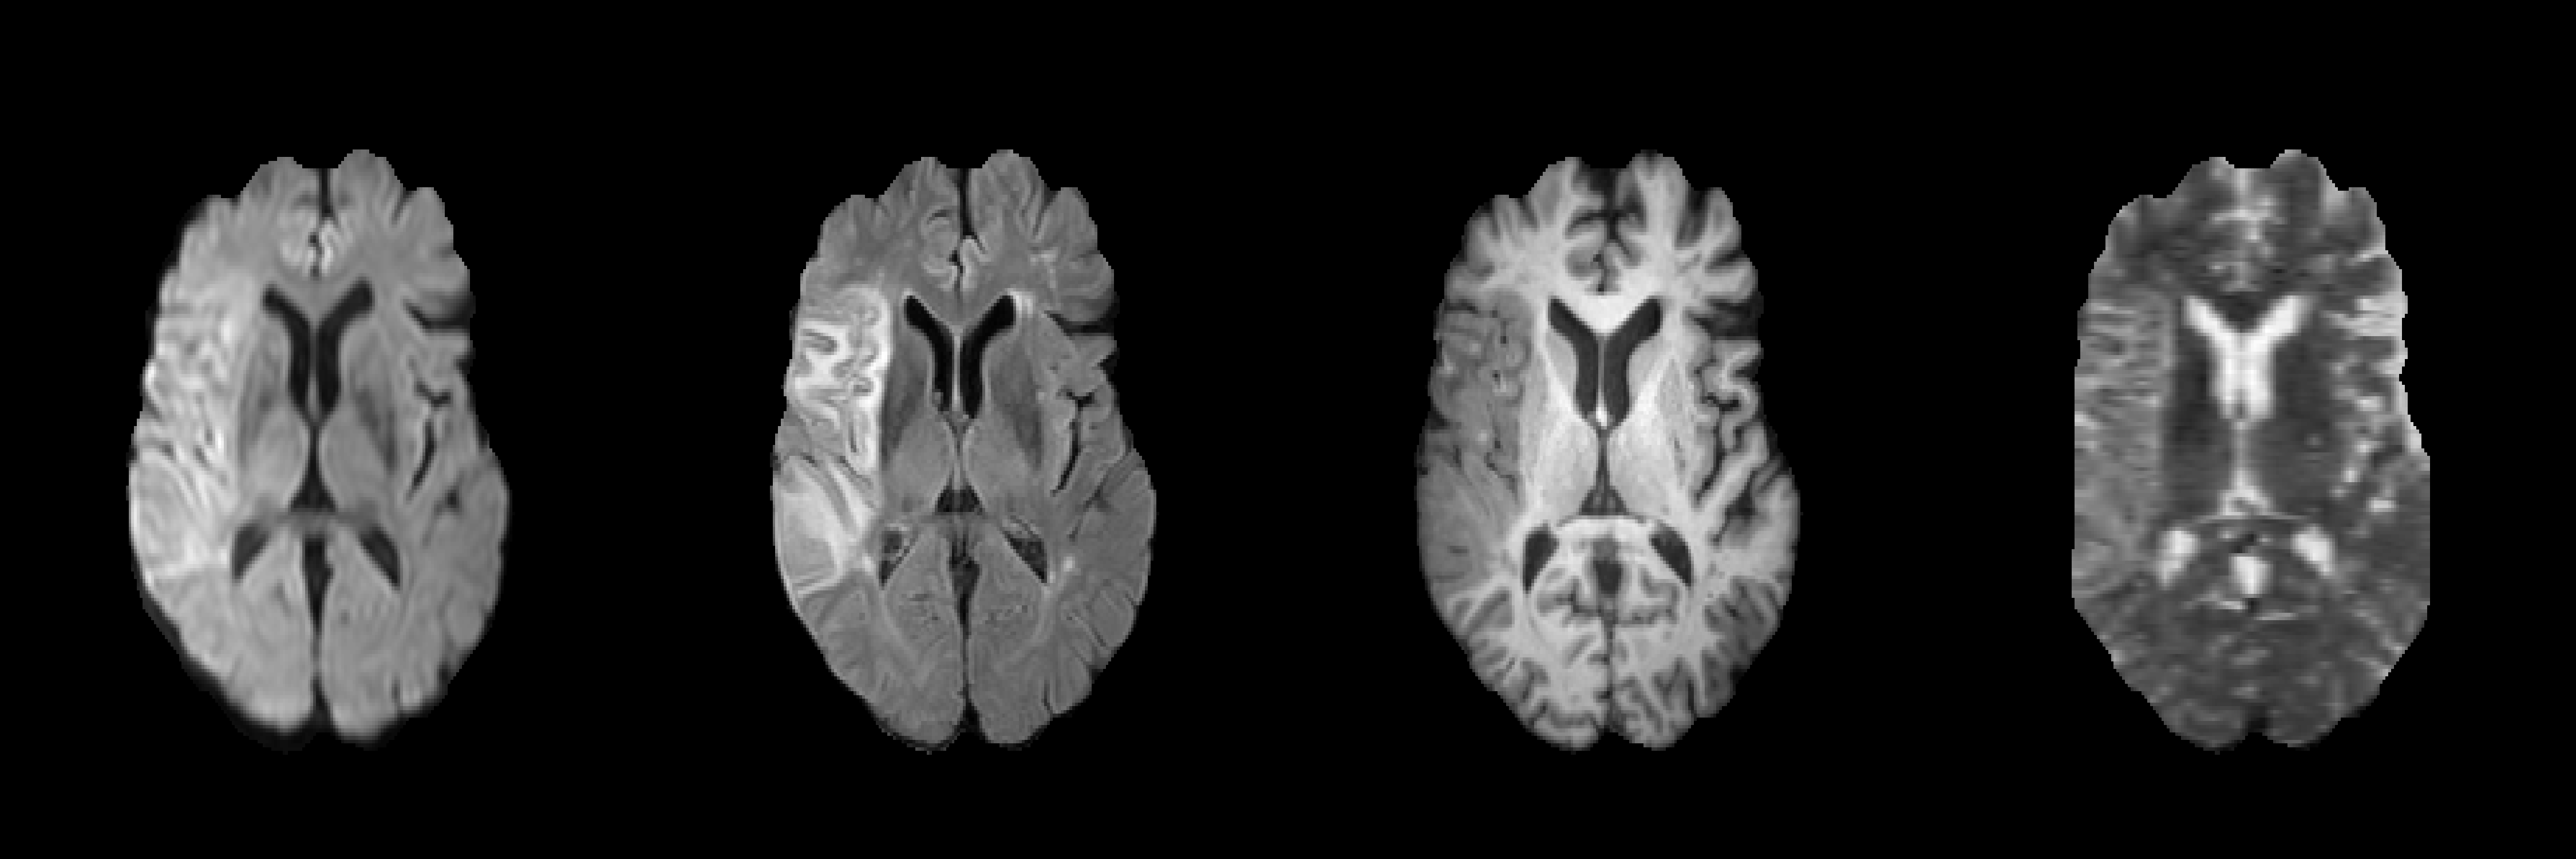
\includegraphics[width=1\linewidth]{image_ex.pdf}
\captionof{figure}{From left to right: DWI, FLAIR, T1w, and T2w images for Subject 05, 2015 ISLES Challenge}
\end{center}\vspace{.5cm}
\large{\section*{\color{uwred}Objectives}}
\begin{enumerate}
\item  Decompose observed variability images at the population level
\item Describe and quantify the main directions of variation
\item Use these directions of variation to improve segmentation and studies of association with health outcomes.
\end{enumerate}

%----------------------------------------------------------------------------------------
%	MATERIALS AND METHODS
%----------------------------------------------------------------------------------------
\large{\section*{\color{uwred}Materials and Methods}}
\noindent To achieve these objectives we propose to decompose the local variability of various moments of the image intensities: the image intensity, image  intensity square, and so on. Consider the following mock example in 2-D:
\begin{center}\vspace{.25cm}
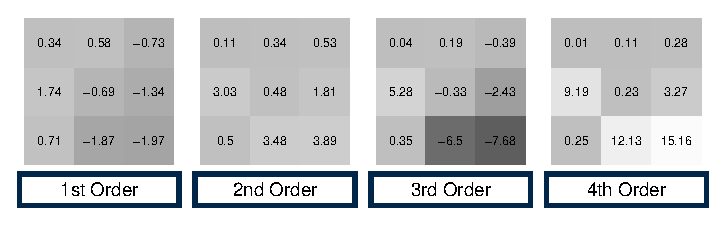
\includegraphics[width=1\linewidth]{ln_example_higherorder_poset.pdf}
\captionof{figure}{2-D mock example of moments of local neighbors}
\end{center}\vspace{.25cm}
\normalsize{
\begin{align*}
\begin{aligned}
X_{ij} = &(0.34, 0.58, \ldots, -1.97, 0.11, \ldots, 3.89, 0.04, \ldots, -7.68, 0.01, \ldots, 15.16).
\end{aligned}
\end{align*}}
\large
\noindent This gives the $j$th row for subject $i$. If we are interested in considering additional imaging modalities, we simply add those as additional columns in the matrix. We preform this operation for each voxel for each subject and stack these vectors into a (potentially large) matrix $\mathbf{X}$. Next,

\begin{itemize}
\item  Center and scale the columns of $\mathbf{X}$
\item Perform PCA on centered and scaled matrix.
\item Calculate principal component scores 
\item Use principal component scores as predictors and expert manual segmentation as outcomes to train a model to perform segmentation
\end{itemize}
\large{\section*{\color{uwred}Computational Issues}}
\noindent Since the size of the matrix $\mathbf{X}$ is large, we need to decompose this matrix without loading it into memory. To overcome this challenge, we iteratively read in each subject and calculate sufficient statistics for the principal component analysis of the correlation matrix between the columns of $\mathbf{X}$. This is implemented in the R package MEDALS (Memory Efficient Decomposition for Analysis of Local neighborhood moments for Segmentation) and is available at https://github.com/JMMaronge/medals.
\vspace{.5cm}
%--------------------------------------------------------------------------------------
%	RESULTS 
%----------------------------------------------------------------------------------------

\large{\section*{\color{uwred}Results}}
\noindent All data shown are from the 2015 ISLES SISS Challenge. Below we show partial ROC (pROC) curves for each subject, as well as overall training and overall testing results. We also show an example of how we performed on a particular subject.

\begin{center}\vspace{.5cm}
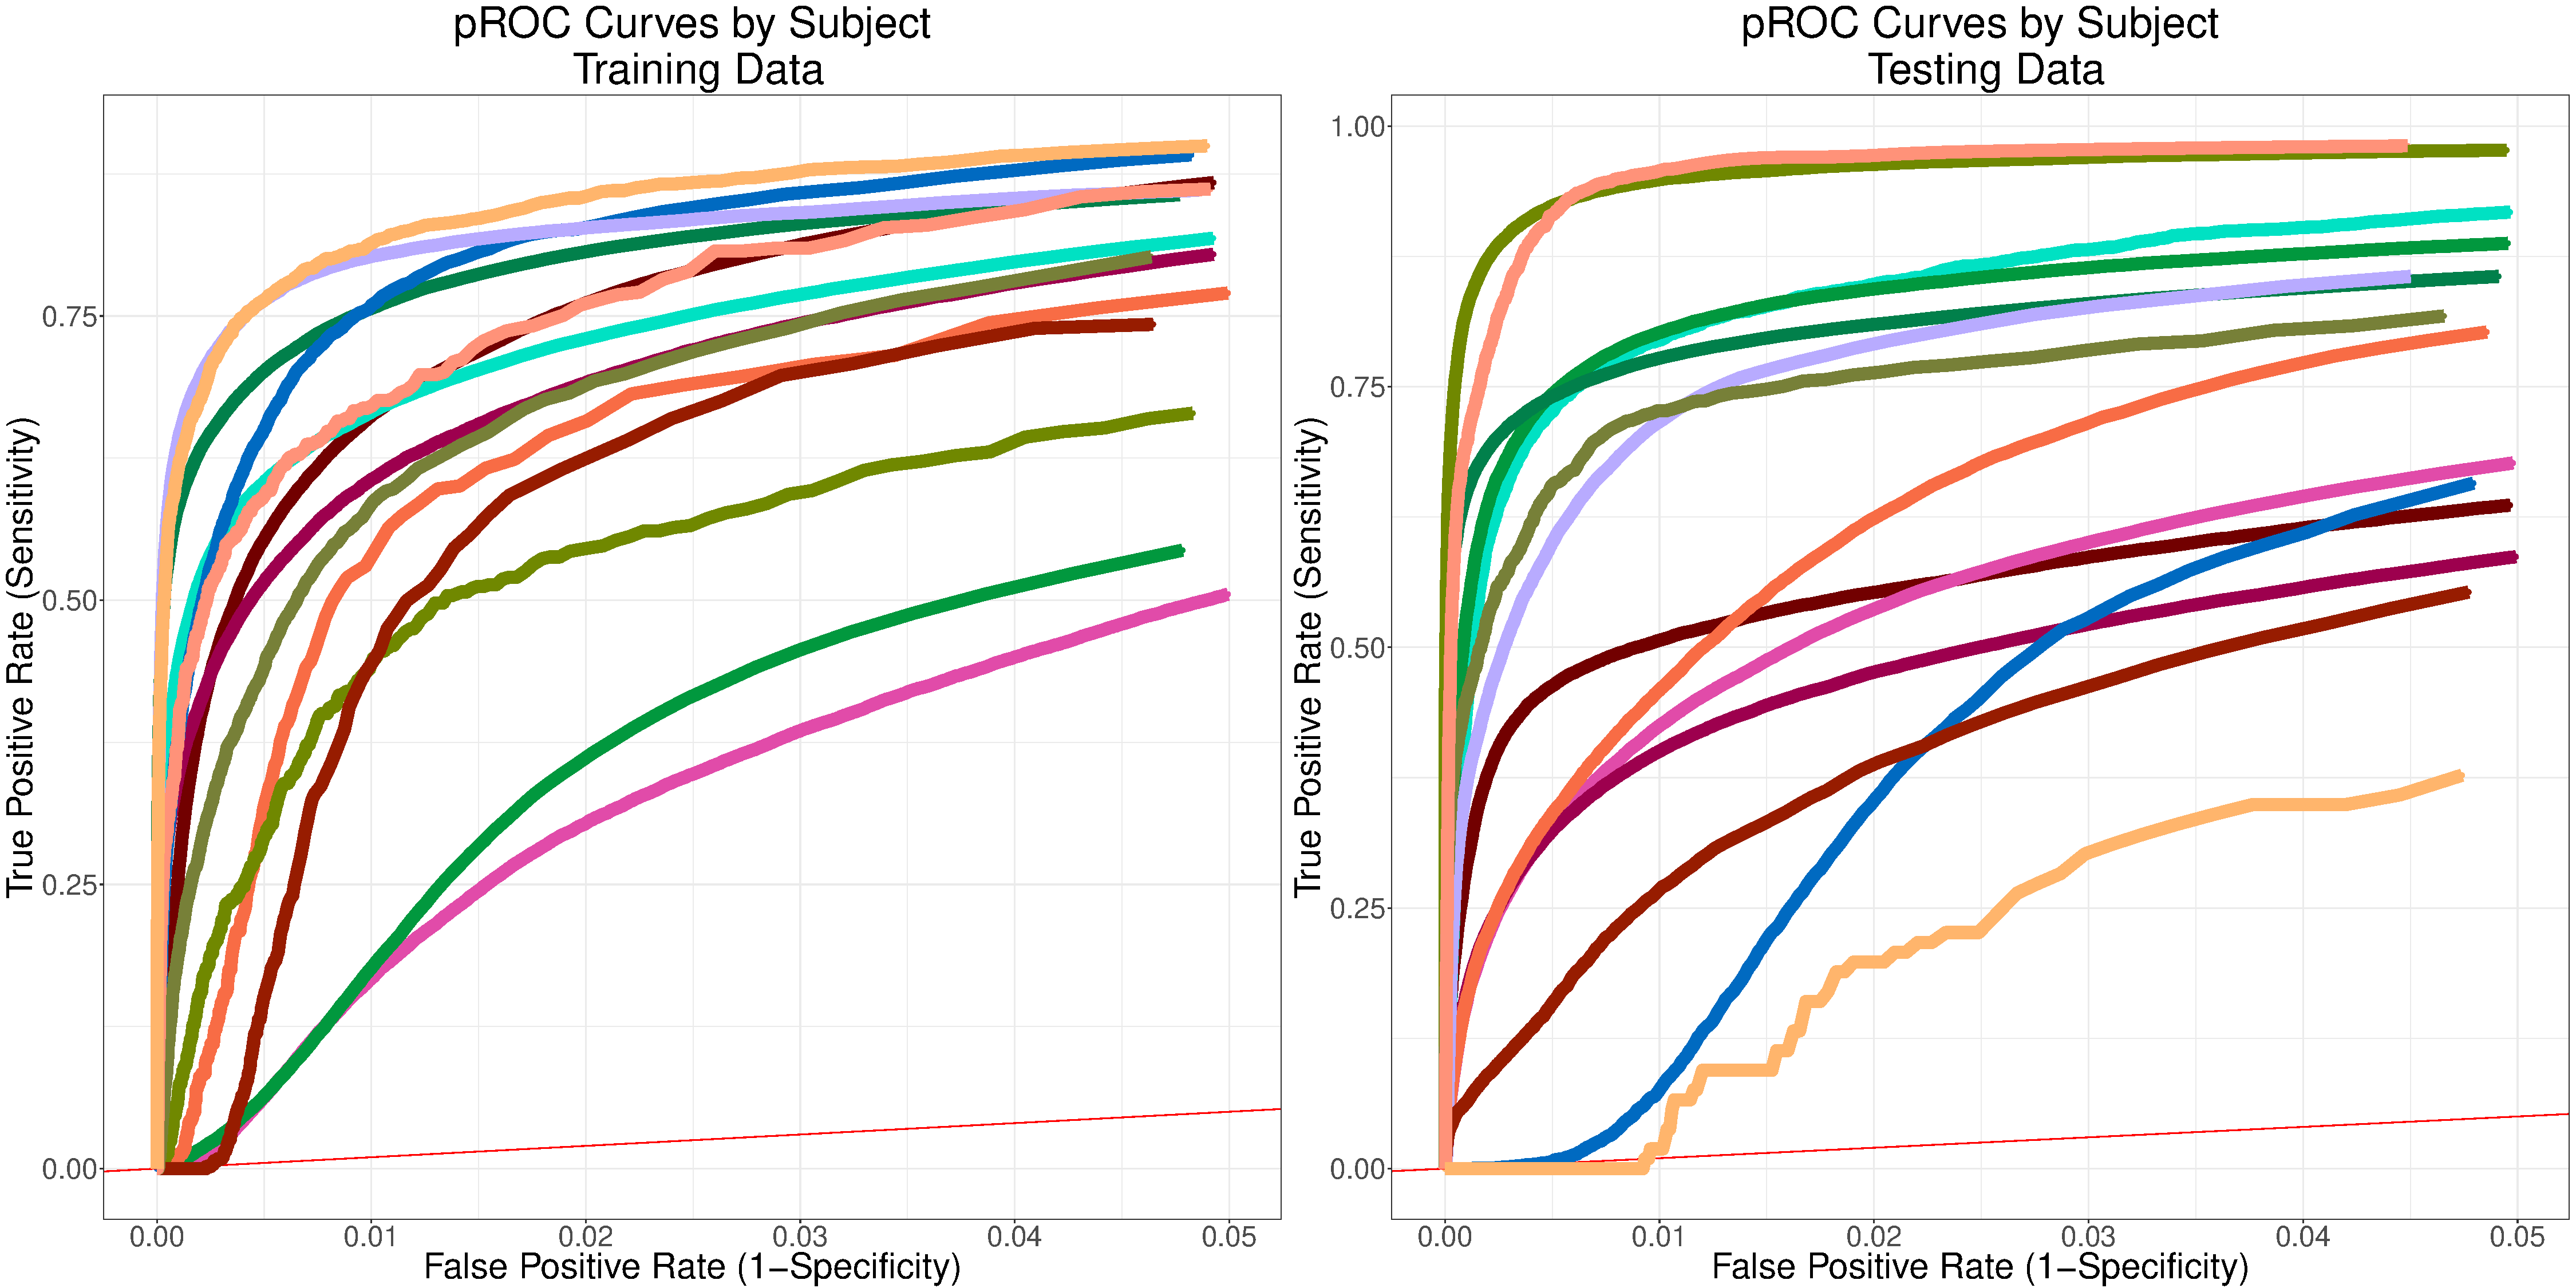
\includegraphics[width=1\linewidth]{procbysubject.pdf}
\captionof{figure}{Subject level pROC curves for training set and testing set}
\end{center}\vspace{.5cm}

\begin{center}\vspace{.5cm}
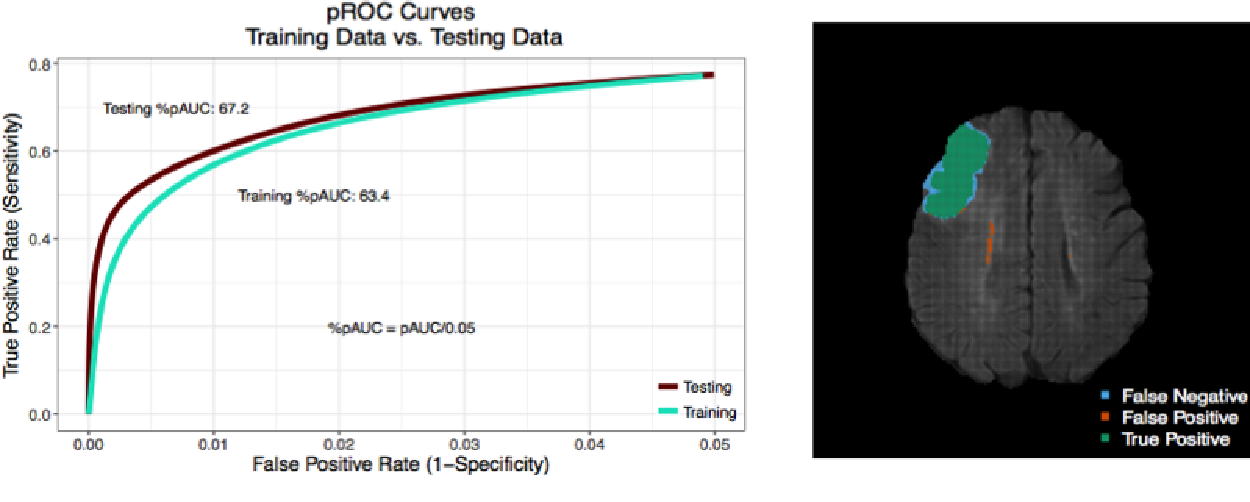
\includegraphics[width=1\linewidth]{bothplots.pdf}
\captionof{figure}{(left) Overall training results and overall testing results (right) Example of performance on one subject}
\end{center}\vspace{.5cm}

\large{\section*{\color{uwred}Conclusions}}
\begin{itemize}
\item  Carefully using information contained within neighborhoods allows for a richer insight of imaging data structures.
\item Using local neighborhoods creates difficulties with storing the data, but these can be overcome by leveraging structure of the data.
\item Characterizing variation in neighborhoods allows for interesting applications in studies of association with health outcomes 
\end{itemize}
\end{multicols}
\end{document}

